\documentclass[12pt]{report}

\usepackage[utf8]{inputenc}
\usepackage[T1]{fontenc}
\usepackage[a4paper, top=2.5cm, bottom=2.5cm, left=3cm, right=2.5cm]{geometry}
\usepackage[ngerman]{babel}
\usepackage{graphicx}
\graphicspath{{images/}}
\usepackage{fancyhdr}
\usepackage{booktabs}
\usepackage[hidelinks]{hyperref}
\usepackage{float}
\usepackage{xcolor}
\usepackage{tabularx}
\usepackage{array}
\usepackage{amsmath}
\usepackage{enumitem}
\usepackage{mdframed}
\usepackage{tocbibind}
\usepackage{caption}
\usepackage{longtable}
\usepackage[htt]{hyphenat}
\usepackage{listings}

\definecolor{thm_green}{RGB}{128,186,36}
\definecolor{light_gray}{RGB}{245,245,245}
\definecolor{warn_orange}{RGB}{200,120,0}

\lstset{
  basicstyle=\ttfamily\footnotesize,
  breaklines=true,
  frame=single,
  backgroundcolor=\color{light_gray},
  showstringspaces=false,
  numbers=left,
  numberstyle=\tiny\color{gray},
  xleftmargin=1.5em,
}

\newcommand{\reporttype}{Projektarbeit}
\newcommand{\semester}{WS 2025/2026}
\newcommand{\reporttitle}{Entwicklung, Integration und Validierung einer ROS2-basierten Hinderniserkennung mit Reaktionsstrategie für automatisierte Modellfahrzeuge}
\newcommand{\authorone}{Aly Elbermawy (5335848)}
\newcommand{\authortwo}{Omar Elalami (5379642)}
\newcommand{\authorthree}{Zakaria Elaboudi (5223183)}
\newcommand{\supervisor}{Prof.\ Dr.\ Benedikt Lattke}
%%\newcommand{\university}{Technische Hochschule Mittelhessen}
\newcommand{\location}{Friedberg}

\makeatletter
\def\@makechapterhead#1{%
  \vspace*{0pt}
  {\raggedright\Huge\bfseries\color{thm_green}\thechapter\quad\normalcolor #1\par\vskip8pt
  \hrule height 1.5pt \vskip12pt}
}
\makeatother

\linespread{1.25}

\pagestyle{fancy}
\fancyhf{}
\fancyhead[L]{\small\nouppercase{\leftmark}}
\fancyhead[R]{\small\thepage}
\renewcommand{\headrulewidth}{0.4pt}

\begin{document}

\begin{titlepage}
\centering

\includegraphics[width=0.42\textwidth]{thm}\\[1.5cm]

{\Large\textbf{\reporttype}}\\[0.3cm]
{\normalsize Fachbereich M -- Master Maschinenbau Mechatronik \quad|\quad \semester}\\[1.5cm]

\begin{center}
    {\large\textbf{\reporttitle}}
\end{center}

\vfill
\begin{tabular}{@{}ll}
\textbf{Autoren:}     & \authorone \\
                      & \authortwo \\
                      & \authorthree \\[0.5em]
\textbf{Betreuer:}    & \supervisor \\[0.5em]
%\textbf{Hochschule:}  & \university, \location \\[0.5em]
\textbf{Abgabedatum:} & \today
\end{tabular}
\vfill
\end{titlepage}

\chapter*{Kurzfassung}
\addcontentsline{toc}{chapter}{Kurzfassung}

Im Rahmen dieser Projektarbeit wurde ein scan-basierter \emph{Follow-the-Gap}-Stack (FTG) für das MXCarkit entwickelt, in die bestehende ROS~2-Fahrzeugarchitektur integriert und experimentell validiert. Das Fahrzeug basiert auf einer Jetson-Plattform, verwendet einen 2D-LiDAR als primäre Sensorik für die lokale Umfelderfassung und wird über eine Ackermann-Steuerkette mit VESC angesteuert. Ziel der Arbeit war es, einen robusten, modularen und sicher testbaren Datenpfad von \texttt{/scan} bis zur autonomen Ausgabe \texttt{/autonomous/ackermann\_cmd} bereitzustellen und dessen Funktionsfähigkeit unter realen Randbedingungen nachzuweisen.

Die realisierte Hauptarchitektur besteht aus vier funktional getrennten Stufen: einer LiDAR-Vorverarbeitung mit TF-basierter Rezentrierung und frontaler Sichtfeldselektion, dem reaktiven C++-Kern \texttt{follow\_the\_gap\_v0} zur Bestimmung einer befahrbaren Lücke, einer Planner-Stufe zur Begrenzung des Lenkwinkels und zur adaptiven Geschwindigkeitswahl sowie einer Control-Stufe zur Überführung der Sollwerte in Ackermann-kompatible Fahrbefehle. Damit wurde eine klare Trennung zwischen Wahrnehmung, lokaler Richtungswahl, fahrdynamischer Policy und fahrzeugspezifischer Schnittstelle erreicht. Der frühere Legacy-Pfad über \texttt{obstacle\_substitution} bleibt aus Kompatibilitätsgründen im Repository erhalten, stellt jedoch nicht mehr den primären Laufzeitpfad dar.

Die theoretische Grundlage bildet das Follow-the-Gap-Verfahren nach Sezer und Gokasan, ergänzt durch die CTU-/F1TENTH-Referenzimplementierung und deren Übertragung in eine moderne ROS~2-Umgebung. Auf dieser Basis wird gezeigt, wie ein klassischer lokaler reaktiver Planungsansatz in eine aktuelle modulare Fahrzeugsoftware integriert werden kann, ohne die bestehende Sicherheits- und Steuerlogik des MXCarkit zu umgehen.

Die experimentelle Validierung erfolgte anhand realer Fahrversuche in strukturierten Innenraumszenarien mit statischen Hindernissen und Eckdurchfahrt. Zur Analyse wurden alle relevanten Systemgrößen mit \texttt{rosbag2} aufgezeichnet und sowohl online mit Foxglove als auch offline über Zeitreihenplots und Kenngrößen ausgewertet. Die Ergebnisse zeigen, dass das System Hindernisse grundsätzlich zuverlässig als freie bzw. belegte Bereiche im LiDAR-Scan interpretieren, kollisionsfreie Ausweichmanöver erzeugen und in die bestehende Fahrzeugsteuerung integrieren kann. Gleichzeitig wurde deutlich, dass die Qualität des Fahrverhaltens wesentlich von der Parametrierung abhängt, insbesondere von Sichtfeld, Clearance-Schwellen, Steering-Slowdown und den internen geometrischen FTG-Konstanten. Die Arbeit liefert damit nicht nur einen funktionsfähigen Stack, sondern auch eine systematische Bewertung seiner Leistungsfähigkeit, Robustheit und Grenzen.
\bigskip


\pagenumbering{Roman}
\setcounter{page}{2}
\tableofcontents
\newpage
\listoffigures
\newpage
\listoftables
\newpage

\pagenumbering{arabic}

\chapter{Grundlagen}
\label{ch:grundlagen}

Dieses Kapitel beschreibt die fachlichen und systemtechnischen Grundlagen der
Arbeit. Zuerst wird das MXCK als Zielplattform eingeordnet. Danach werden die
für die Arbeit relevanten ROS~2-Begriffe erklärt. Abschließend wird der
Follow-the-Gap-Algorithmus sowohl in seiner ursprünglichen Form als auch in der
für dieses Projekt relevanten scan-basierten Variante erläutert.

\section{Das MXCarkit als Zielplattform}

Das MXCarkit ist ein Jetson-basiertes, containerisiertes Versuchsfahrzeug für
Lehre und Entwicklung im Bereich autonomer Fahrfunktionen. Laut der aktuellen
MXCK-Dokumentation werden die Systembestandteile bewusst in Docker-Container
aufgeteilt, wobei \texttt{mxck2\_ws} die Kernfunktionalität und
\texttt{development\_ws} experimentelle bzw.\ GPU-nahe Entwicklung aufnimmt.
Die zentrale Startlogik für Sensorik und Aktorik liegt im Paket
\texttt{mxck\_run}; einzelne Teilfunktionen wie LiDAR oder Kamera werden über
Launch-Argumente wie \texttt{run\_lidar:=true} aktiviert.

\begin{table}[H]
\centering
\caption{Relevante MXCK-Systemeigenschaften für diese Arbeit}
\label{tab:mxck_overview}
\begin{tabular}{>{\raggedright\arraybackslash}p{4.2cm} >{\raggedright\arraybackslash}p{9.2cm}}
\toprule
\textbf{Aspekt} & \textbf{Bedeutung für den FTG-Stack} \\
\midrule
NVIDIA Jetson & Rechnerplattform für ROS~2, Paket-Build, Sensorverarbeitung und Debugging \\
Docker-basierter Betrieb & Trennung von Sensor-/Control-Containern und Entwicklungsumgebung \\
2D-LiDAR (\texttt{/scan}) & Primärer Sensor für den reaktiven FTG-Pfad \\
Ackermann-Steuerung & Lenkwinkel- und Geschwindigkeitsvorgaben werden als Ackermann-Befehl ausgegeben \\
Bestehende Fahrzeugsteuerung & Der FTG-Stack darf die vorhandene VESC-/Safety-Kette nicht umgehen \\
\bottomrule
\end{tabular}
\end{table}

Für diese Arbeit ist vor allem wichtig, dass der autonome Output nicht direkt an
VESC-Topics gesendet wird, sondern an
\texttt{/autonomous/ackermann\_cmd}. Dadurch bleibt die bestehende MXCK-
Sicherheits- und Moduslogik erhalten.

\section{ROS~2: Workspace, Paket, Node und Launch}

Da der gesamte Stack auf ROS~2 basiert, ist ein sauberes Verständnis der
Architekturelemente notwendig.

\subsection{Workspace}

Ein ROS~2-Workspace ist ein Verzeichnis, in dem mehrere Pakete gemeinsam
gebaut werden. Gebräuchlich ist die Struktur
\texttt{src/}, \texttt{build/}, \texttt{install/}, \texttt{log/}. Im MXCK-Projekt
wird dieser Aufbau direkt genutzt: \texttt{mxck2\_ws} enthält die
Kernfunktionalität, während \texttt{development\_ws} für zusätzliche
Entwicklungsarbeit vorgesehen ist.

\subsection{Paket}

Ein Paket bündelt eine klar abgegrenzte Funktion. In dieser Arbeit werden
Pakete für Perception, Planner, Control und Bringup verwendet. Für Python-Pakete
sind insbesondere \texttt{package.xml}, \texttt{setup.py},
\texttt{setup.cfg}, der Python-Modulordner und optionale Launch-/Config-Ordner
relevant. Für C++-Pakete kommen stattdessen \texttt{CMakeLists.txt},
\texttt{package.xml}, Header- und Source-Dateien zum Einsatz.

\subsection{Node}

Ein Node ist ein laufender Prozess innerhalb des ROS~2-Graphs. Nodes abonnieren
Topics, veröffentlichen Topics, verwenden Parameter und werden meist über
Launch-Dateien gemeinsam gestartet.

\subsection{Launch-Dateien und YAML-Parameter}

ROS~2 nutzt bevorzugt Python-basierte Launch-Dateien. Diese starten mehrere
Nodes, reichen Parameter weiter und erlauben deklarative Startkonfigurationen.
Für dieses Projekt ist das besonders wichtig, weil die Pipeline nur dann stabil
und reproduzierbar ist, wenn Node-Namen, Executables, YAML-Dateien und Topics
konsistent zusammenpassen.

\section{Follow-the-Gap als reaktiver Planungsansatz}

Der Ursprung des Follow-the-Gap-Verfahrens liegt in der Arbeit von Sezer und
Gokasan. Dort wird FTG als lokaler Hindernisvermeidungsansatz formuliert, der
die Umgebung nur anhand der aktuell sichtbaren Hindernisse bewertet. Statt eine
globale Karte aufzubauen, sucht das Verfahren in jedem Zeitpunkt nach der
größten passierbaren Lücke und richtet das Fahrzeug möglichst auf deren Mitte
aus.

\subsection{Zentrale Idee der Originalarbeit}

Die Originalarbeit beschreibt drei Kernschritte:

\begin{enumerate}[label=\arabic*)]
    \item Aufbau einer Hindernis- bzw.\ Gap-Repräsentation,
    \item Bestimmung eines sicheren Gap-Center-Winkels,
    \item Fusion von Gap-Richtung und Zielrichtung zu einem finalen Heading.
\end{enumerate}

Wesentliche Eigenschaften des Verfahrens sind laut Originalarbeit:
\begin{itemize}
    \item Berücksichtigung des Sichtfelds,
    \item Berücksichtigung nicht-holonomer Fahrdynamik,
    \item keine lokale-Minimum-Problematik wie bei Potentialfeldern,
    \item nur wenige Tuning-Parameter.
\end{itemize}

\subsection{Gap-Idee in vereinfachter Form}

Im klassischen FTG werden aus den Hindernisgrenzen aufeinanderfolgende
``Gaps'' bestimmt. Die größte geeignete Lücke wird ausgewählt. Aus dieser
Lücke wird ein Winkel $\varphi_{gap}$ bestimmt. Anschließend wird dieser mit
einem Zielwinkel $\varphi_{goal}$ fusioniert, wobei nahe Hindernisse den
Einfluss des Gap-Winkels erhöhen und freie Umgebung den Einfluss des
Zielwinkels stärkt.

Formal beschreibt die Originalarbeit die finale Heading-Bildung als gewichtete
Fusion aus Gap-Winkel und Zielwinkel. Entscheidend ist dabei der kleinste
Hindernisabstand $d_{min}$: je kleiner $d_{min}$ ist, desto stärker soll die
Planung sicherheitsorientiert in Richtung des Gaps reagieren.

\subsection{Von der Originalformulierung zur praktischen Scan-Variante}

Die CTU-F1/10-Implementierung übernimmt die FTG-Idee in einen ROS-Node
\texttt{follow\_the\_gap}. Dessen klassischer ROS-Eingang ist ein
\texttt{sensor\_msgs/LaserScan} auf \texttt{/scan}; als Zielwinkel kann
optional \texttt{/lsr/angle} vorgegeben werden. Als wesentliche Ausgänge nennt
das CTU-Repository \texttt{/final\_heading\_angle},
\texttt{/visualize\_final\_heading\_angle},
\texttt{/visualize\_obstacles} und
\texttt{/visualize\_largest\_gap}.

Für das MXCK-Projekt wird dieser Kerngedanke nicht als
\texttt{/scan}-Direkteingang verwendet, sondern als \emph{scan-basierter
Vorverarbeitungspfad}:

\begin{lstlisting}
 /scan
   -> scan_preprocessor_node
   -> /autonomous/ftg/scan_filtered
   -> follow_the_gap_v0 (input_mode=scan)
   -> /final_heading_angle
   -> /gap_found
\end{lstlisting}

Damit wird der eigentliche C++-Planerkern entlastet: Das Re-Centering auf die
Fahrzeugfront, die Clipping-Logik und die Front-Clearance-Bestimmung finden
bereits vorher statt.

\section{Warum ROS~2 für dieses Thema relevant ist}

Die CTU-Arbeit von Endler zeigt, warum ROS~2 im Kontext schneller
autonomer Fahrfunktionen relevant ist. Zentrale Punkte sind:
\begin{itemize}
    \item DDS-basierte Kommunikation statt ROS~1-Master-Modell,
    \item klare Trennung von \texttt{rcl}, \texttt{rmw} und DDS,
    \item Build-System \texttt{ament} mit \texttt{colcon},
    \item moderne Python-Launchfiles,
    \item bessere Grundlage für Messung von Latenzen, Jitter und
    End-to-End-Ketten.
\end{itemize}

Für diese Projektarbeit ist das vor allem deshalb wichtig, weil das MXCK nicht
nur einen Algorithmus ``irgendwie ausführt'', sondern als Prozesskette aus
mehreren ROS~2-Nodes verstanden werden muss. Schon kleine Inkonsistenzen in
Topic-Namen, QoS, Frames oder Startreihenfolge können das Gesamtsystem
unbrauchbar machen.

\section{Zusammenfassung}

Die theoretische Grundlage dieser Arbeit ist damit zweigeteilt:
Einerseits liefert die FTG-Originalliteratur die mathematische und
planungslogische Basis. Andererseits liefert der aktuelle ROS~2-/F1TENTH-
Kontext die technische Form, in der diese Idee heute auf einem Jetson-basierten
Lehrfahrzeug umgesetzt wird. Genau an dieser Schnittstelle setzt die
vorliegende Arbeit an.

\chapter{Systembeschreibung und Durchführung}
\label{ch:durchfuehrung}

Dieses Kapitel beschreibt die konkret umgesetzte Systemarchitektur sowie die methodische Durchführung der Implementierung und Validierung des Follow-the-Gap-Stacks im Repository \texttt{ftg\_mxck}. Der Fokus liegt auf dem scan-basierten Hauptpfad, der als primäre Laufzeitarchitektur definiert wurde.

\section{Gesamtarchitektur des Systems}

Die entwickelte Pipeline folgt einer strikt modularen Struktur, die sich in vier logisch getrennte Verarbeitungsebenen gliedert:

\begin{enumerate}
    \item LiDAR-Vorverarbeitung (Perception)
    \item Reaktiver Planerkern (Follow-the-Gap)
    \item Policy-basierte Entscheidungslogik (Planner)
    \item Fahrzeugschnittstelle (Control)
\end{enumerate}

Die resultierende Datenflusskette ist in Abbildung~\ref{fig:system_pipeline} dargestellt.

\begin{figure}[H]
    \centering
    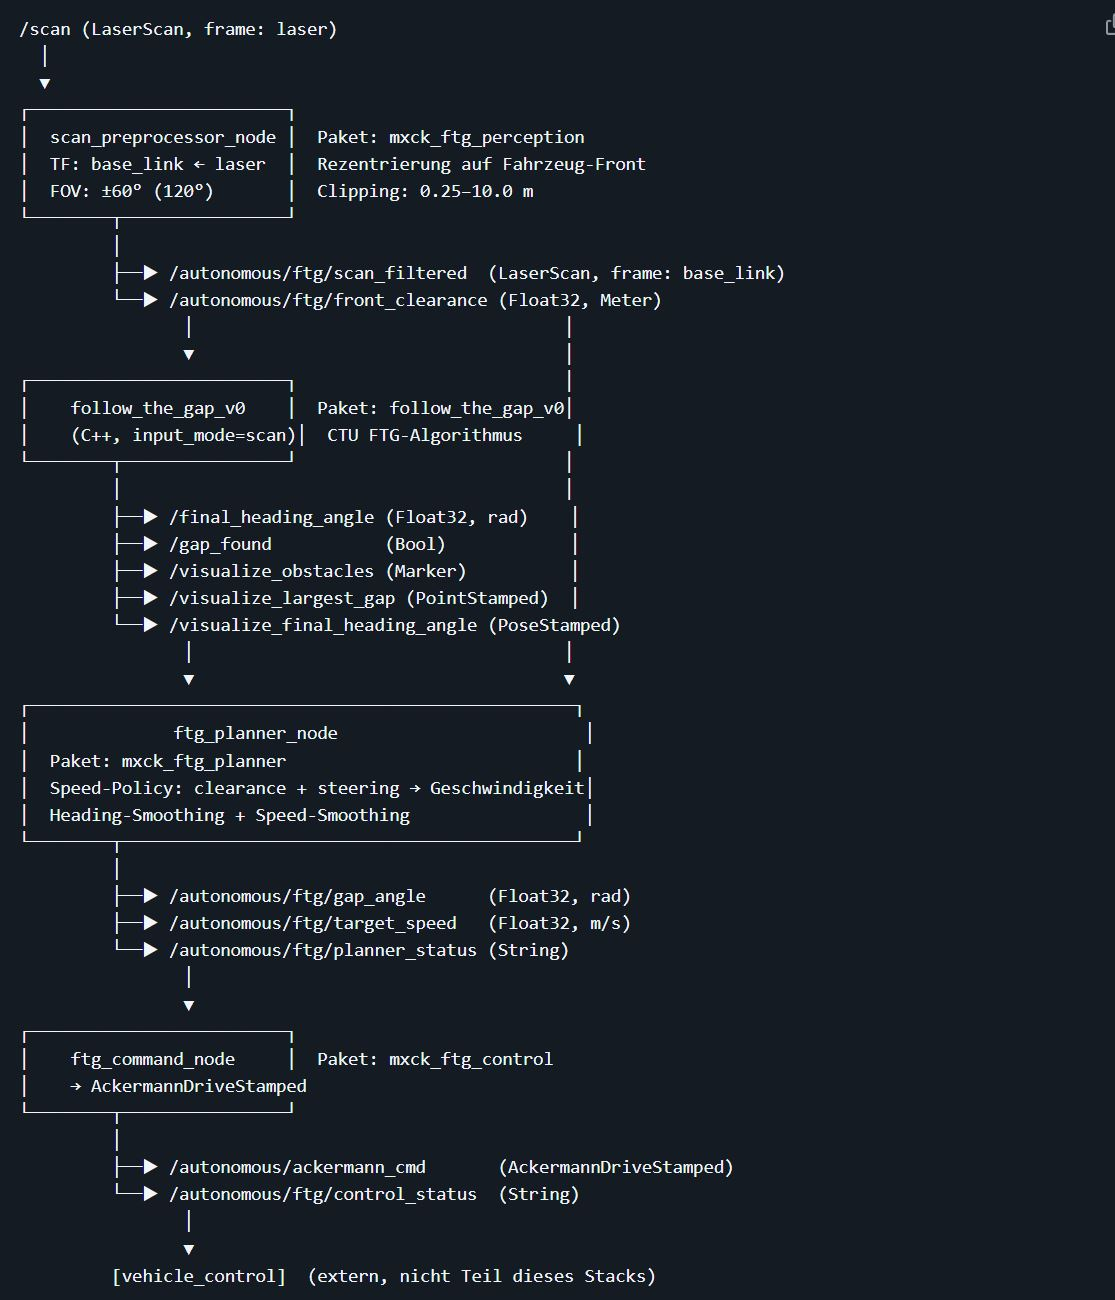
\includegraphics[width=0.85\textwidth]{images/Gesamtarch.JPG}
    \caption{Gesamtarchitektur des scan-basierten FTG-Stacks . Die Pipeline reicht vom Rohscan bis zur Ackermann-Ausgabe und zeigt die klare Trennung zwischen Wahrnehmung, Planung und Steuerung.\cite{mxck_repo}}
    \label{fig:system_pipeline}
\end{figure}

Der vollständige Aufbau sowie alle Konfigurationsdateien sind im Repository \texttt{ftg\_mxck} dokumentiert. Im Rahmen dieser Arbeit wird auf eine vollständige Reproduktion aller Startbefehle verzichtet; stattdessen wird die Architektur konzeptionell beschrieben und auf die implementierten Komponenten verwiesen.

\section{Algorithmische Grundlage}

Der eingesetzte Planungsansatz basiert auf dem Follow-the-Gap-Verfahren nach Sezer und Gokasan~\cite{sezer2012}. Die konkrete Implementierung orientiert sich an der F1TENTH-/CTU-Referenz~\cite{ctu_ftg} und wurde unverändert als C++-Kern in den Stack integriert.

\begin{figure}[H]
    \centering
    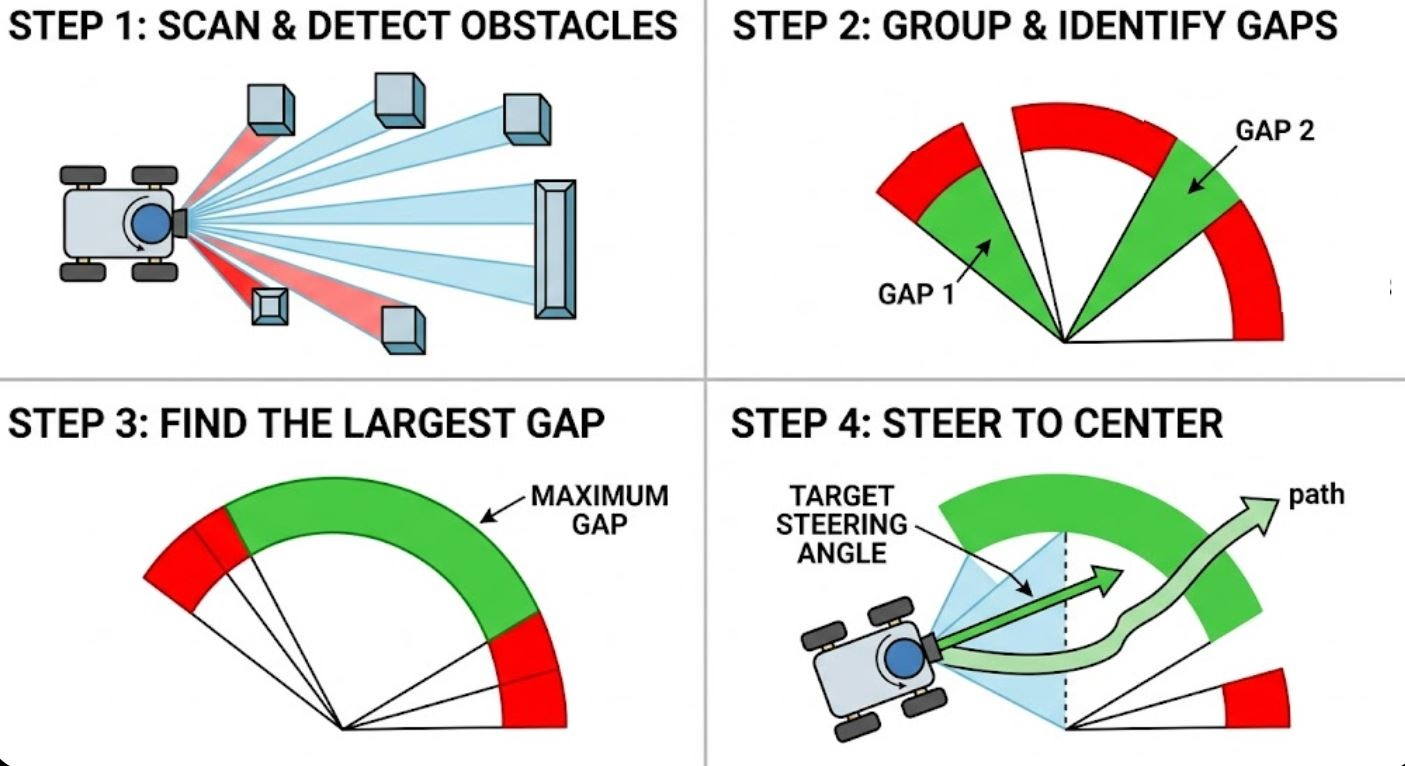
\includegraphics[width=1\textwidth]{images/ftg_algorithm1.JPG}
    \caption{Schematische Darstellung des Follow-the-Gap-Prinzips \cite{ai2026}.}
    \label{fig:ftg_algorithm}
\end{figure}

Die zentrale Idee besteht darin, aus einem eindimensionalen Distanzprofil die größte kollisionsfreie Lücke zu bestimmen und das Fahrzeug entlang deren Mittelpunkt auszurichten. Diese Strategie ermöglicht eine robuste reaktive Navigation ohne globale Karteninformation.

\section{Stufe 1: LiDAR-Vorverarbeitung}

Die Vorverarbeitung transformiert den Rohscan in eine für den FTG-Kern geeignete Repräsentation.

\subsection{Funktionale Aufgaben}

Die implementierte Verarbeitung umfasst:

\begin{itemize}
    \item Transformation des Scans in den Fahrzeugrahmen mittels TF,
    \item Definition eines frontalen Sichtfensters,
    \item Entfernung ungültiger Messwerte,
    \item Glättung des Signals zur Rauschreduktion,
    \item Berechnung des minimalen Frontabstands.
\end{itemize}

Diese Schritte sind notwendig, um die geometrische Konsistenz zwischen Sensor und Fahrzeug sicherzustellen.

\subsection{Node Perception Erklärung}
Bla Bla Bla

\section{Stufe 2: Follow-the-Gap-Kern}

Der Planerkern bildet das algorithmische Zentrum des Systems. Er verarbeitet den vorbereiteten Scan und berechnet daraus einen Richtungswinkel.

\subsection{Verarbeitungsschritte}

Innerhalb des Algorithmus erfolgen:

\begin{enumerate}
    \item Identifikation von Hindernisbereichen,
    \item Bestimmung zusammenhängender freier Bereiche (Gaps),
    \item Auswahl des größten befahrbaren Gaps,
    \item Berechnung eines Zielwinkels innerhalb dieses Gaps.
\end{enumerate}

\subsection{Ausgabegrößen}

Der Algorithmus liefert:

\begin{itemize}
    \item einen kontinuierlichen Heading-Winkel,
    \item ein binäres Signal zur Gap-Erkennung.
\end{itemize}

Diese Ausgabe ist bewusst fahrzeugagnostisch gehalten und enthält keine Informationen über Geschwindigkeit oder Dynamik.

\section{Stufe 3: Planner}

Der Planner interpretiert die algorithmische Ausgabe im Kontext der Fahrzeugdynamik und Sicherheitsanforderungen.

\subsection{Funktionale Rolle}

Im Gegensatz zum FTG-Kern handelt es sich hierbei nicht um einen Planungsalgorithmus im engeren Sinne, sondern um eine Entscheidungslogik, die folgende Aufgaben übernimmt:

\begin{itemize}
    \item Validierung der Eingangsdaten (Freshness),
    \item Begrenzung des Lenkwinkels,
    \item adaptive Geschwindigkeitswahl in Abhängigkeit vom Frontabstand,
    \item Zustandsbewertung des Systems.
\end{itemize}

\subsection{Interpretation der Sensordaten}

Die Geschwindigkeit wird als Funktion des minimalen Abstands gewählt. Dabei gilt:

\begin{itemize}
    \item große Abstände $\rightarrow$ hohe Geschwindigkeit,
    \item kleine Abstände $\rightarrow$ reduzierte Geschwindigkeit,
    \item kritische Abstände $\rightarrow$ Stopp.
\end{itemize}

Diese Policy stellt sicher, dass der reaktive Charakter des FTG-Ansatzes nicht zu unsicheren Fahrzuständen führt.

\section{Stufe 4: Control}

Die letzte Stufe des Systems übernimmt die Transformation der Planner-Ausgabe in fahrzeugspezifische Steuerbefehle.

\subsection{Aufgabe}

Die berechneten Sollwerte werden in ein Ackermann-kompatibles Nachrichtenformat überführt und an die bestehende Fahrzeugsteuerung übergeben.

\subsection{Systemintegration}

Ein wesentliches Designkriterium ist, dass die bestehende Sicherheits- und Steuerlogik des MXCarkit unverändert bleibt. Der entwickelte Stack liefert ausschließlich Sollwerte und greift nicht direkt in die Aktorik ein.

\section{Versuchsdurchführung}

Die Validierung des Systems erfolgte anhand realer Fahrversuche im Innenraum.

\subsection{Versuchsaufbau}

Die Tests wurden in einem strukturierten Korridor durchgeführt, der durch gezielt platzierte Hindernisse definiert wurde.

\begin{figure}[H]
    \centering
    % PLACEHOLDER: Teststrecke 1
    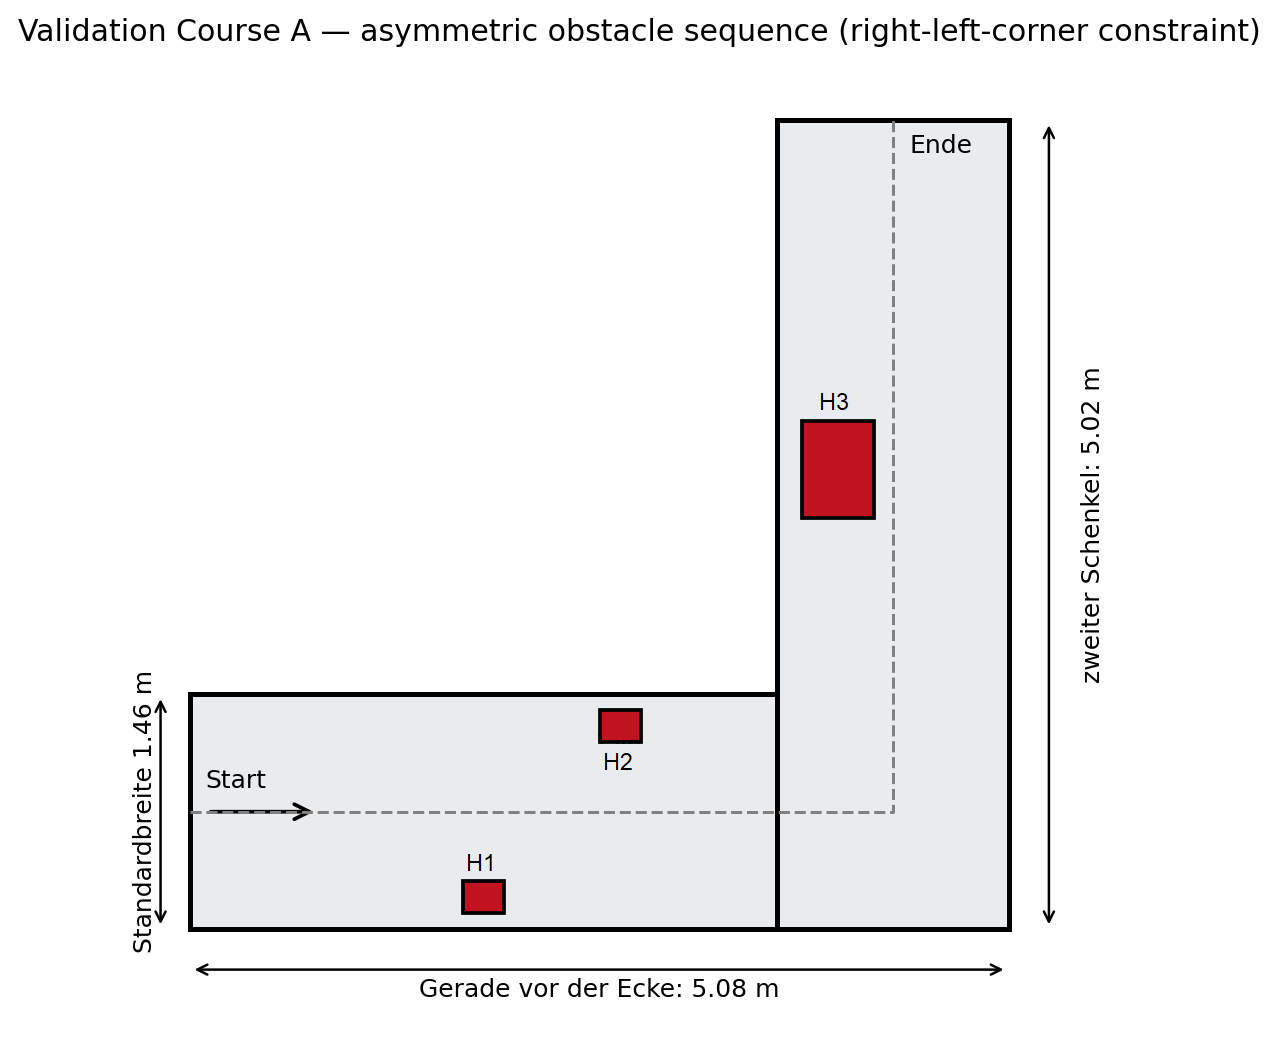
\includegraphics[width=0.75\textwidth]{images/validation_course_A_schematic.png}
    \caption{Versuchsaufbau Aufnahme 1: Korridor mit einem statischen Hindernis.}
    \label{fig:test_track1}
\end{figure}

\begin{figure}[H]
    \centering
    % PLACEHOLDER: Teststrecke 2
    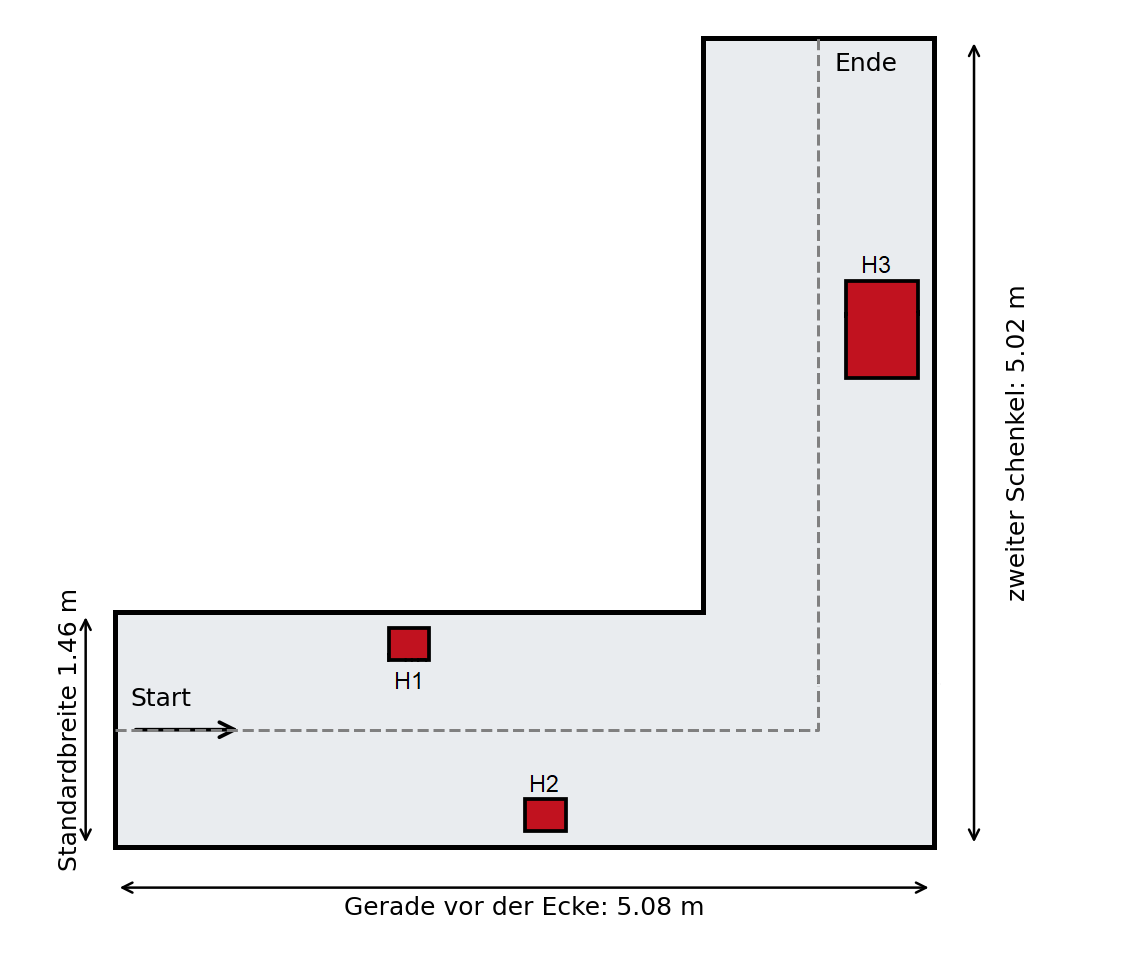
\includegraphics[width=0.75\textwidth]{images/validation_course_B_schematic.png}
    \caption{Versuchsaufbau Aufnahme 2: Mehrere Hindernisse und dynamische Veränderung der Umgebung.}
    \label{fig:test_track2}
\end{figure}
\subsection{Parametrierung des Systems}
\label{sec:parametrierung_system}

Die Validierungsfahrten wurden mit einer fest definierten Konfiguration des FTG-Stacks durchgeführt. 
Die Parametrierung ist für die Bewertung des Systemverhaltens von zentraler Bedeutung, da sie sowohl die 
geometrische Interpretation der Umgebung als auch die resultierende Fahrdynamik direkt beeinflusst. 
Insbesondere wirken sich Sichtfeld, Distanzgrenzen, Geschwindigkeitsgrenzen sowie die Abbremslogik 
unmittelbar auf das Ausweich- und Kurvenverhalten des Fahrzeugs aus.

Tabelle~\ref{tab:ftg_runtime_parameter} fasst die im Validierungsbetrieb verwendeten Laufzeitparameter 
der drei zentralen Softwarestufen Perception, Planner und Control zusammen.

\renewcommand{\arraystretch}{1.2}
\begin{longtable}{p{2.6cm} p{3.0cm} p{1.8cm} p{6.2cm}}
\caption{Verwendete Laufzeitparameter des FTG-Stacks während der Validierungsfahrten.}
\label{tab:ftg_runtime_parameter}\\
\toprule
\textbf{Stufe / Node} & \textbf{Parameter} & \textbf{Wert} & \textbf{Bedeutung und Einfluss auf das Fahrverhalten} \\
\midrule
\endfirsthead

\toprule
\textbf{Stufe / Node} & \textbf{Parameter} & \textbf{Wert} & \textbf{Bedeutung und Einfluss auf das Fahrverhalten} \\
\midrule
\endhead

Perception & \texttt{front\_center\_deg} & 0.0 & Definition der Fahrtrichtung im \texttt{base\_link}-Frame; die physische LiDAR-Montage wird über TF berücksichtigt. \\
Perception & \texttt{front\_fov\_deg} & 180.0 & Breite des für FTG verwendeten Sichtfensters; größere Werte erhöhen die Umgebungsabdeckung, lassen aber seitliche Wände stärker in die Entscheidungsfindung einfließen. \\
Perception & \texttt{clip\_min\_range\_m} & 0.25 & Untere Distanzgrenze; unterdrückt sehr nahe Punkte und mögliche Eigenreflexionen des Fahrzeugs. \\
Perception & \texttt{clip\_max\_range\_m} & 10.0 & Obere Distanzgrenze; begrenzt die Auswertung auf den relevanten Messbereich. \\
Perception & \texttt{enable\_moving\_average} & \texttt{true} & Aktiviert eine Glättung des Distanzsignals zur Reduktion einzelner Ausreißer. \\
Perception & \texttt{moving\_average\_window} & 3 & Fenstergröße der Mittelung; größere Werte erhöhen die Glättung, reduzieren aber die Reaktivität. \\

Planner & \texttt{input\_timeout\_sec} & 0.50 & Maximales Alter der Eingangsdaten; bei Überschreitung wird aus Sicherheitsgründen gestoppt. \\
Planner & \texttt{max\_abs\_gap\_angle\_rad} & 0.45 & Begrenzung des resultierenden Lenkwinkels. \\
Planner & \texttt{cruise\_speed\_mps} & 0.45 & Maximale Sollgeschwindigkeit bei freier Umgebung. \\
Planner & \texttt{min\_speed\_mps} & 0.20 & Untergrenze der Fahrgeschwindigkeit im normalen Betrieb. \\
Planner & \texttt{stop\_speed\_mps} & 0.00 & Sollgeschwindigkeit im Stoppfall. \\
Planner & \texttt{stop\_clearance\_m} & 0.25 & Kritischer Frontabstand, unterhalb dessen das Fahrzeug anhalten soll. \\
Planner & \texttt{caution\_clearance\_m} & 0.50 & Abstand, ab dem wieder die volle Clearance-Freigabe erreicht wird. \\
Planner & \texttt{steering\_slowdown\_start\_rad} & 0.40 & Ab diesem Lenkwinkel wird die Geschwindigkeit schrittweise reduziert. \\
Planner & \texttt{steering\_slowdown\_full\_rad} & 0.70 & Lenkwinkelbereich für maximale Geschwindigkeitsreduktion; bewusst größer als der maximal zulässige Gap-Winkel gewählt, um Corner-Blockaden zu vermeiden. \\
Planner & \texttt{heading\_smoothing\_alpha} & 0.4 & Glättungsfaktor für den Heading-Winkel; reduziert sprunghafte Richtungswechsel zwischen aufeinanderfolgenden Scans. \\
Planner & \texttt{speed\_smoothing\_alpha} & 0.3 & Glättungsfaktor für die Beschleunigungsphase; Bremsvorgänge bleiben davon unberührt und werden direkt umgesetzt. \\

Control & \texttt{input\_timeout\_sec} & 0.50 & Sicherheitsgrenze für veraltete Planner-Daten; bei Überschreitung wird ein Nullkommando ausgegeben. \\
Control & \texttt{angle\_to\_steering\_gain} & -1.00 & Vorzeichen- und Skalierungsfaktor für die Lenkabbildung; negative Werte invertieren die physische Lenkreaktion. \\
Control & \texttt{max\_steering\_angle\_rad} & 0.45 & Hardwarebedingte Begrenzung des Lenkwinkels. \\
Control & \texttt{min\_speed\_mps} & 0.18 & Untere Grenze der ausgegebenen Sollgeschwindigkeit. \\
Control & \texttt{max\_speed\_mps} & 1.80 & Obergrenze der ausgegebenen Sollgeschwindigkeit. \\
\bottomrule
\end{longtable}

Neben den Laufzeitparametern verwendet der C++-Kern \texttt{follow\_the\_gap\_v0} zusätzlich interne,
nicht zur Laufzeit parametrierbare Geometrie- und Gewichtungskonstanten. Diese sind in
Tabelle~\ref{tab:ftg_internal_constants} zusammengefasst, da sie die Passierbarkeit von Lücken und
damit das resultierende Fahrverhalten ebenfalls wesentlich beeinflussen.


\begin{table}[H]
\centering
\caption{Interne FTG-Konstanten des C++-Kerns \texttt{follow\_the\_gap\_v0}.}
\label{tab:ftg_internal_constants}
\begin{tabularx}{\textwidth}{l l X}
\toprule
\textbf{Konstante} & \textbf{Wert} & \textbf{Bedeutung} \\
\midrule
\texttt{kCarRadius} & 0.40 m & Effektiver Sicherheitsradius zur Hindernis-Aufblähung und damit maßgeblich für die als passierbar bewertete Gap-Breite. \\
\texttt{kTurnRadius} & 0.30 m & Modellannahme für die Kurvenfähigkeit des Fahrzeugs. \\
\texttt{kTrackMinWidth} & 0.35 m & Mindestbreite für bestimmte Corner- und Gap-Bewertungen. \\
\texttt{kDistanceToCorner} & 0.22 m & Sicherheitsabstand bei Corner-bezogenem Verhalten. \\
\texttt{kGapWeightCoefficient} & 100.0 & Gewichtung der Gap-Richtung in der Zielrichtungsbestimmung. \\
\texttt{kCornerWeightCoefficient} & 100.0 & Gewichtung corner-spezifischer Anteile in der Zielwahl. \\
\bottomrule
\end{tabularx}
\end{table}

Die tabellarische Zusammenstellung ist für die Reproduzierbarkeit der Ergebnisse essenziell, da bereits
moderate Änderungen einzelner Parameter zu deutlich unterschiedlichem Fahrverhalten führen können. 
Insbesondere das Sichtfeld, die Clearance-Schwellen sowie der effektive Fahrzeugradius beeinflussen, 
ob enge Passagen als befahrbar oder blockiert interpretiert werden.

\subsection{Messmethodik und Datenerfassung}
\label{sec:messmethodik}

Zur experimentellen Bewertung des Systems wurden sämtliche relevanten Systemgrößen während der Fahrt
zeitlich synchron aufgezeichnet und anschließend offline ausgewertet. Die Datenerfassung erfolgte mit
\texttt{rosbag2}, sodass sowohl Rohdaten als auch Zwischen- und Ausgangsgrößen des gesamten FTG-Stacks
reproduzierbar analysiert werden konnten.

Die Auswertung fokussierte sich auf vier zentrale Beobachtungsgrößen:

\begin{itemize}
    \item \textbf{Distanzverlauf:} Charakterisierung der Umgebungssituation über den gefilterten Scan sowie den minimalen Frontabstand,
    \item \textbf{Heading-Winkel:} Bewertung der vom FTG-Kern bestimmten Zielrichtung und deren Weiterverarbeitung im Planner,
    \item \textbf{Geschwindigkeit:} Analyse der Sollgeschwindigkeit des Planners und der tatsächlich ausgegebenen Ackermann-Geschwindigkeit,
    \item \textbf{Gap-Erkennung:} Bewertung, ob und wie stabil freie, befahrbare Lücken detektiert wurden.
\end{itemize}

Die aufgezeichneten Topics deckten sowohl den sensorischen Eingang als auch alle relevanten
Zwischenstufen des Verarbeitungsgraphen ab. Tabelle~\ref{tab:recorded_topics} zeigt die
für die Validierung herangezogenen Nachrichtenströme.

\begin{table}[H]
\centering
\caption{Für die Validierung aufgezeichnete Topics des FTG-Stacks.}
\label{tab:recorded_topics}
\begin{tabular}{p{5.2cm} p{3.2cm} p{6.0cm}}
\toprule
\textbf{Topic} & \textbf{Nachrichtentyp} & \textbf{Funktion in der Auswertung} \\
\midrule
\texttt{/scan} & \texttt{sensor\_msgs/LaserScan} & Rohdaten des LiDARs als Eingangssignal \\
\texttt{/autonomous/ftg/scan\_filtered} & \texttt{sensor\_msgs/LaserScan} & vorverarbeiteter, rezentrierter Scan für FTG \\
\texttt{/autonomous/ftg/front\_clearance} & \texttt{std\_msgs/Float32} & minimaler Frontabstand als Eingangsgröße der Speed-Policy \\
\texttt{/final\_heading\_angle} & \texttt{std\_msgs/Float32} & vom FTG-Kern berechnete Zielrichtung \\
\texttt{/gap\_found} & \texttt{std\_msgs/Bool} & binäre Information über erkannte befahrbare Lücken \\
\texttt{/autonomous/ftg/gap\_angle} & \texttt{std\_msgs/Float32} & begrenzter Planner-Lenkwinkel \\
\texttt{/autonomous/ftg/target\_speed} & \texttt{std\_msgs/Float32} & vom Planner berechnete Sollgeschwindigkeit \\
\texttt{/autonomous/ackermann\_cmd} & \texttt{ackermann\_msgs/AckermannDriveStamped} & tatsächlich ausgegebener Fahrbefehl \\
\texttt{/autonomous/ftg/planner\_status} & \texttt{std\_msgs/String} & textuelle Zustandsdiagnose des Planners \\
\texttt{/autonomous/ftg/control\_status} & \texttt{std\_msgs/String} & textuelle Zustandsdiagnose der Control-Stufe \\
\texttt{/visualize\_obstacles} & \texttt{visualization\_msgs/Marker} & Visualisierung erkannter Hindernispunkte \\
\texttt{/visualize\_largest\_gap} & \texttt{geometry\_msgs/PointStamped} & Visualisierung der größten detektierten Lücke \\
\texttt{/visualize\_final\_heading\_angle} & \texttt{geometry\_msgs/PoseStamped} & Visualisierung der resultierenden Fahrtrichtung \\
\texttt{/tf}, \texttt{/tf\_static} & \texttt{tf2\_msgs/TFMessage} & geometrische Referenz zwischen Sensor- und Fahrzeugrahmen \\
\bottomrule
\end{tabular}
\end{table}

Zur Online-Beobachtung des Systemzustands wurde zusätzlich \textit{Foxglove Studio} eingesetzt.
Die Live-Visualisierung diente insbesondere der Plausibilitätsprüfung von Scan, Heading, Gap-Erkennung,
Planner-Zuständen und Ackermann-Ausgabe während der Testdurchführung. Abbildung~\ref{fig:foxglove_validation}
zeigt exemplarisch ein für die Validierung verwendetes Layout mit 3D-Ansicht, Statusmeldungen und
zeitbasierten Signalverläufen.

\begin{figure}[H]
    \centering
    % PLACEHOLDER: Foxglove-Screenshot einfügen
    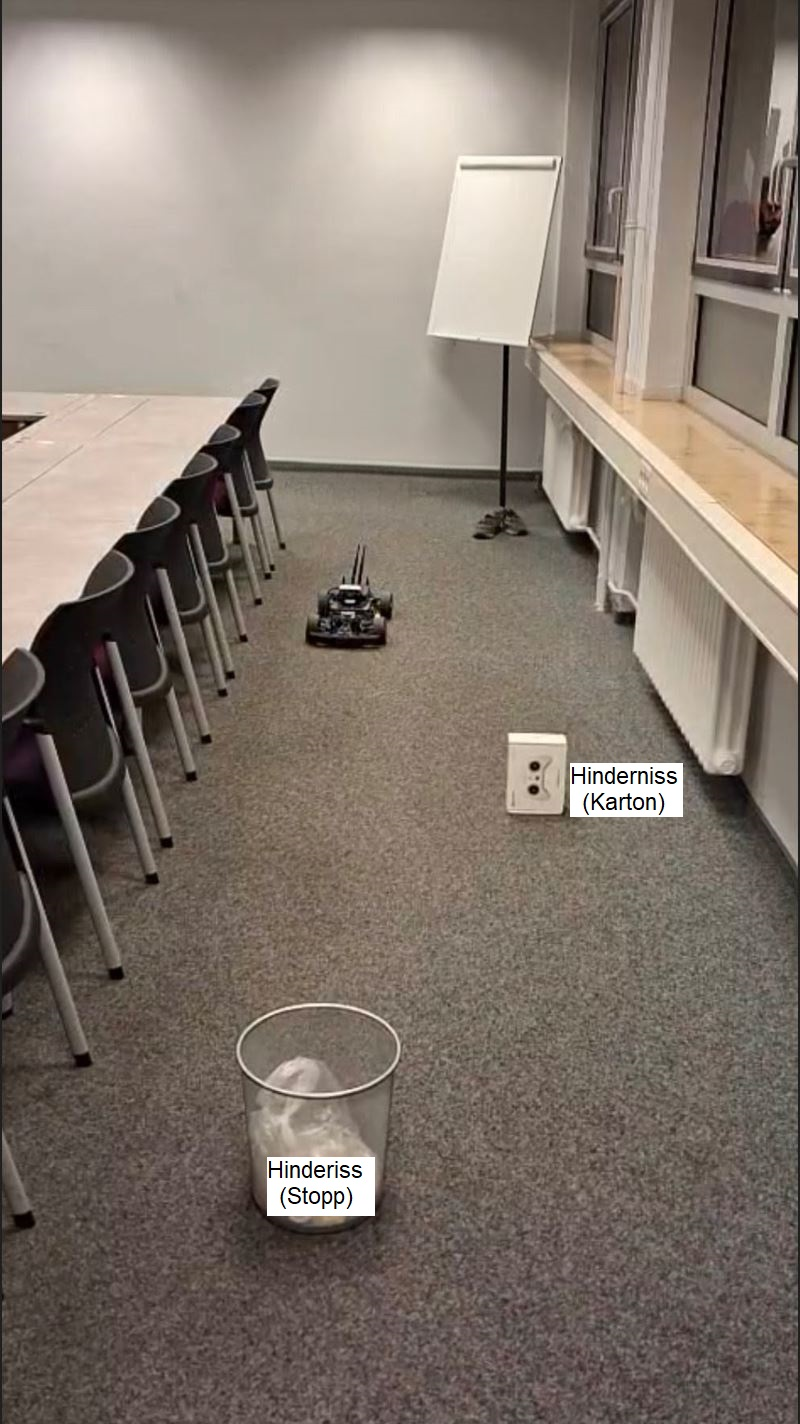
\includegraphics[width=0.95\textwidth]{images/foxglove_validation_overview.png}
    \caption{Exemplarisches Foxglove-Layout zur Online-Beobachtung des FTG-Stacks während der Validierungsfahrten. Dargestellt sind Sensorik, Visualisierungstopics und zentrale Zustandsgrößen des Planungs- und Steuerpfads.}
    \label{fig:foxglove_validation}
\end{figure}

Die eigentliche quantitative Bewertung erfolgte auf Basis der aufgezeichneten Bags in einer
anschließenden Offline-Analyse. Hierzu wurden die Signalverläufe der beiden Validierungsläufe
zeitlich ausgewertet und in Form von Metriken und Zeitreihenplots aufbereitet. Zu den
wesentlichen Kenngrößen zählen unter anderem:

\begin{itemize}
    \item mittlerer und minimaler Frontabstand,
    \item mittlere Sollgeschwindigkeit und Zeitanteil mit Stopp-Anforderung,
    \item Zeitanteil mit erfolgreicher Gap-Erkennung,
    \item Auftreten von Sättigungen im Heading- bzw. Gap-Winkel,
    \item Auftreten von Planner-Zuständen wie \textit{normal}, \textit{stale} oder \textit{no valid gap found}.
\end{itemize}

Die daraus resultierenden Validierungsplots und metrischen Vergleiche werden in Kapitel~\ref{ch:diskussion}
zur Diskussion und Bewertung der beiden Teststrecken herangezogen.

\chapter{Diskussion und Bewertung}
\label{ch:diskussion}

Dieses Kapitel bewertet die entwickelte Systemarchitektur hinsichtlich ihrer technischen Eignung, Robustheit und Übertragbarkeit. Dabei werden sowohl algorithmische als auch systemtechnische Aspekte analysiert.

\section{Bewertung der gewählten Gesamtarchitektur}

Die Entscheidung für eine strikt scan-basierte Pipeline stellt eine bewusste Abkehr von komplexeren, mehrstufigen Wahrnehmungsansätzen dar. Diese Reduktion des Datenpfads führt zu mehreren signifikanten Vorteilen.

\subsection{Reduktion von Komplexität}

Durch den direkten Übergang von \texttt{/scan} zu einer gefilterten Scan-Repräsentation wird auf zusätzliche Abstraktionsebenen wie Objektextraktion oder Hindernismodellierung verzichtet. Dies reduziert:

\begin{itemize}
    \item die Anzahl potenzieller Fehlerquellen,
    \item den Parametrierungsaufwand,
    \item die Latenz innerhalb der Verarbeitungskette.
\end{itemize}

Gerade für reaktive Verfahren wie Follow-the-Gap ist diese Vereinfachung fachlich sinnvoll, da der Algorithmus explizit für rohnahe Sensordaten formuliert wurde~\cite{sezer2012}.

\subsection{Vergleich mit alternativen Ansätzen}

Im Gegensatz zu globalen Planern oder kartengestützten Verfahren besitzt der implementierte Stack keine Kenntnis über die Umgebung außerhalb des aktuellen Sichtfelds. Dies führt zu folgenden Konsequenzen:

\begin{itemize}
    \item hohe Reaktionsfähigkeit auf lokale Hindernisse,
    \item jedoch eingeschränkte Fähigkeit zur global optimalen Pfadplanung.
\end{itemize}

Die Architektur ist daher klar als \textbf{lokaler reaktiver Planer} einzuordnen und nicht als vollständiges Navigationssystem.



\section{Analyse der Planner- und Control-Schicht}

Die Trennung zwischen algorithmischem Kern, Planner und Control stellt eine klare funktionale Hierarchie dar.

Die gewählte Aufteilung ermöglicht:

\begin{itemize}
    \item Wiederverwendbarkeit des FTG-Kerns,
    \item unabhängige Anpassung der Fahrstrategie,
    \item klare Definition von Verantwortlichkeiten innerhalb der Pipeline.
\end{itemize}

Insbesondere fungiert der Planner als \textbf{Policy-Schicht}, die sicherstellt, dass die reaktive Planung in physikalisch realisierbare und sichere Fahrbefehle überführt wird.


\section{Bewertung der experimentellen Ergebnisse}

Die durchgeführten Fahrversuche zeigen, dass das System in strukturierten Innenräumen grundsätzlich funktionsfähig ist, jedoch klare Abhängigkeiten von der Umgebungskonfiguration aufweist.

\subsection{Quantitativer Vergleich der Validierungsläufe}

Tabelle~\ref{tab:validierung_vergleich} fasst die wichtigsten Metriken der beiden Testläufe zusammen.

\begin{table}[H]
\centering
\caption{Vergleich der Metriken: Validierung Test 1 vs. Test 2}
\label{tab:validierung_vergleich}
\begin{tabular}{l c c}
\toprule
\textbf{Metrik} & \textbf{Test 1} & \textbf{Test 2} \\
\midrule
Gap erkannt & 90\% & 56\% \\
Speed = 0 (Zeitanteil) & 10\% & 44\% \\
$\emptyset$ Geschwindigkeit & 0,37 m/s & 0,40 m/s \\
Min. Clearance & 0,27 m & 0,34 m \\
Kollisionen & 0 & 0 \\
Heading-Bereich & $\pm$ 0,8 rad & $\pm$ 0,8 rad \\
\midrule
\bottomrule
\end{tabular}
\end{table}

\subsection{Detailbewertung der Szenarien}

\begin{itemize}
    \item \textbf{Test 1:} Alle Hindernisse wurden umfahren und die 90°-Ecke gemeistert. Der kurze Stopp an der Ecke resultiert aus dem \texttt{kCarRadius}-Parameter von 0,4\,m, der hier eine konservative Reaktion auslöste.
    \item \textbf{Test 2:} Dieser Lauf ist als eingeschränkt zu bewerten. Ein Zeitanteil von 44\% mit Geschwindigkeit 0 sowie eine Gap-Erkennungsrate von nur 56\% weisen auf Instabilitäten hin. Die Ursache liegt im 180° FOV, das zu breit gewählt war, wodurch Seitenwände die Lückenerkennung störten.
\end{itemize}

\subsection{Empfehlungen aus der Validierung}
Bewertung für alle Parameter.
Basierend auf den Ergebnissen wird empfohlen, das FOV auf 120° zurückzusetzen, um Störeinflüsse durch Wände zu minimieren. Zudem sollte der \texttt{kCarRadius} von 0,4\,m auf 0,20\,m reduziert werden, um dem realen 30\,cm breiten Fahrzeug besser gerecht zu werden.

\subsection{Robustheit gegenüber statischen Hindernissen}

In beiden Versuchsreihen konnte das Fahrzeug Hindernisse erkennen und geeignete Ausweichbewegungen berechnen. Die Anpassung der Geschwindigkeit in Abhängigkeit vom Frontabstand erwies sich als stabil und reproduzierbar.

\subsection{Verhalten bei dynamischen Änderungen}

Besonders relevant ist das Verhalten bei der Entfernung eines Hindernisses während der Fahrt. Hier zeigt sich ein charakteristischer Vorteil reaktiver Systeme:

\begin{itemize}
    \item sofortige Anpassung an die neue Umgebung,
    \item keine Notwendigkeit zur Replanung einer globalen Route.
\end{itemize}

Dieses Verhalten bestätigt die Eignung des FTG-Ansatzes für dynamische Szenarien.

\subsection{Grenzfälle}

Trotz der positiven Ergebnisse treten typische Einschränkungen auf:

\begin{itemize}
    \item keine strategische Entscheidung in Sackgassen,
    \item potenziell suboptimale Pfadwahl in komplexen Geometrien,
    \item Abhängigkeit von Sichtfeldbegrenzungen.
\end{itemize}

Diese Einschränkungen sind inhärent im Algorithmus begründet und nicht als Implementierungsfehler zu interpretieren.

\section{Einordnung in den wissenschaftlichen Kontext}

Die Kombination aus klassischem FTG-Ansatz~\cite{sezer2012}, CTU-Referenzimplementierung~\cite{ctu_ftg} und moderner ROS~2-Infrastruktur~\cite{ros2_docs} zeigt, wie etablierte Verfahren in aktuelle Softwarearchitekturen überführt werden können.

Die vorliegende Arbeit leistet dabei keinen Beitrag zur Weiterentwicklung des Algorithmus selbst, sondern zur:

\begin{itemize}
    \item systematischen Integration,
    \item reproduzierbaren Umsetzung,
    \item technischen Konsolidierung eines bestehenden Ansatzes.
\end{itemize}


\chapter{Fazit und Ausblick}
\label{ch:fazit}

% ============================================================
\section{Fazit}
% ============================================================

Diese Projektarbeit dokumentiert den vollständigen Entwicklungs-,
Integrations- und Evaluationsprozess eines Follow-the-Gap-basierten
Hindernisvermeidungssystems für das MXCarkit.

Das gesetzte Ziel -- ein Fahrzeug, das selbstständig Hindernisse
erkennt, ausweicht und bei unausweichlichen Hindernissen anhält --
konnte im Rahmen der durchgeführten Experimente \emph{nur
teilweise} erreicht werden. Die Einzelkomponenten des Stacks
(LiDAR-Empfang, Hinderniskonvertierung, Planerkern, Geschwindigkeitsadapter
und Ackermann-Ausgabe) funktionierten im Einzeltest korrekt.
Im Zusammenspiel verhinderten jedoch systemische Fehler
die kollisionsfreie Navigation.

\textbf{Zu den wesentlichen Erkenntnissen dieser Arbeit zählen:}

\begin{itemize}
    \item \textbf{Kalibrierung ist entscheidend:} Der Parameter
    \texttt{front\_center\_deg} hatte enormen Einfluss auf das
    Gesamtverhalten. Eine Abweichung von nur $45°$ (von $135°$ auf $90°$)
    führte dazu, dass der Algorithmus konstant am Grenzwert operierte
    und keinerlei situationsabhängige Reaktion zeigte.

    \item \textbf{TF-Infrastruktur ist nicht optional:}
    Reaktive Planungsalgorithmen hängen fundamental von der korrekten
    räumlichen Zuordnung der Sensordaten ab. Das Fehlen der
    \texttt{base\_link}$\to$\texttt{laser}-Transformation verhinderte
    eine automatische, robuste Kalibrierung und war die tiefste
    Ursache des Systemversagens.

    \item \textbf{Hindernismodellierung beeinflusst Lückenbewertung:}
    Ein Sicherheitsradius von $0{,}01$\,m ist für ein Fahrzeug
    der Breite $>30$\,cm unzureichend. Die Wahl des Hindernisradius
    direkt beeinflusst, welche Lücken als passierbar gelten.

    \item \textbf{Modularität erleichtert Debugging:}
    Die konsequent modulare Paketstruktur mit dedizierten
    Debug-Topics (\texttt{/visualize\_obstacles},
    \texttt{/autonomous/ftg/planner\_status}) ermöglichte eine
    systematische Eingrenzung der Fehlerquellen -- ohne diese
    Transparenz wäre das Debugging erheblich schwieriger gewesen.

    \item \textbf{Container-Grenzen sind ROS-Grenzen:}
    Das DDS-basierte Kommunikationsmodell von ROS~2 funktioniert
    gut innerhalb eines Netzwerks, jedoch entstehen durch
    unterschiedliche ROS~2-Versionen und QoS-Inkompatibilitäten
    unsichtbare Kommunikationsgrenzen.
\end{itemize}

% ============================================================
\section{Ausblick}
% ============================================================

Mit den in Kapitel~\ref{ch:diskussion} beschriebenen
Korrekturen ist zu erwarten, dass das System die ursprüngliche
Zielsetzung -- kollisionsfreies Fahren mit Nothalt --
vollständig erfüllen kann. Über die unmittelbaren Korrekturen
hinaus bieten sich folgende Erweiterungen an:

\begin{enumerate}
    \item \textbf{Clustering-Integration:}
    Ein DBSCAN-basierter Clusteringschritt zwischen
    \texttt{obstacle\_substitution} und dem Planerkern
    würde die Hindernisrepräsentation erheblich verbessern
    und das beobachtete Zickzack-Lenkverhalten reduzieren.

    \item \textbf{Systematische Parametrierung via Rosbag:}
    Die aufgezeichneten Rosbags können für offline
    Parametertests genutzt werden, ohne das reale
    Fahrzeug jedes Mal neu starten zu müssen.

    \item \textbf{Foxglove-Dashboard:}
    Eine Foxglove-Konfiguration mit 3D-Panel
    (Hindernisvisualisierung, Heading-Pfeil),
    Plot-Panel (\texttt{/final\_heading\_angle},
    \texttt{/gap\_found}) und Raw-Messages-Panel
    würde zukünftige Kalibrierung und Diagnose
    erheblich erleichtern.

    \item \textbf{Streckentest:}
    Erprobung des Systems auf einer definierten
    Teststrecke mit bekannten Hindernishindernissen
    in verschiedenen Konfigurationen (Engstellen,
    L-Kurven, dynamische Hindernisse).

    \item \textbf{Geschwindigkeitsskalierung:}
    Nach erfolgreicher Kollisionsfreiheit kann
    die \texttt{cruise\_speed} schrittweise erhöht
    und die Geschwindigkeitsstufen feinjustiert werden.
\end{enumerate}


\begin{thebibliography}{99}
%\addcontentsline{toc}{chapter}{Literaturverzeichnis}

\bibitem{sezer2012}
Sezer, V.; Gokasan, M.:
\textit{A Novel Obstacle Avoidance Algorithm: ``Follow the Gap Method''}.
Robotics and Autonomous Systems, Vol. 60, No. 9, 2012, pp. 1123--1134.
DOI: 10.1016/j.robot.2012.05.021.

\bibitem{endler2022}
Endler, M.:
\textit{Using ROS 2 for High-Speed Maneuvering in Autonomous Driving}.
Bachelor’s Thesis, Czech Technical University in Prague, 2022.

\bibitem{ctu_ftg}
Czech Technical University – Intelligent and Interactive Graphics Group (CTU-IIG):
\textit{F1TENTH Follow-the-Gap Implementation (f1t-ftg)}.
Available at: \url{https://github.com/CTU-IIG/f1t-ftg}
(Accessed: 2026-04).

\bibitem{f1tenth}
O’Kelly, M. et al.:
\textit{F1TENTH: An Open-Source Evaluation Environment for Continuous Control and Reinforcement Learning}.
NeurIPS Workshop on Machine Learning for Autonomous Driving, 2019.

\bibitem{ros2_docs}
Open Robotics:
\textit{ROS 2 Documentation}.
Available at: \url{https://docs.ros.org}
(Accessed: 2026-04).

\bibitem{ai2026}
Gemini 3 Flash et al.:
\textit{KI-generierte Foto}.
Erstellt am 12. April 2026.
Software: ChatGPT und Google AI.

\bibitem{mxck_repo}
Elalami, O. et al.:
\textit{ftg\_mxck – ROS 2 Follow-the-Gap Stack for MXCarkit}.
GitHub Repository.
Available at: \url{https://github.com/OmarMElalami/ftg_mxck}
(Accessed: 2026-04).

\bibitem{mxck_ws}
MXCK Platform:
\textit{mxck2\_ws – ROS 2 Workspace for MXCarkit}.
Available at: \url{https://github.com/william-mx/mxck2_ws}
(Accessed: 2026-04).

\end{thebibliography}

\end{document}
